\section{HARP extension for flexible performance-complexity balancing}\label{sec:our-method}

Graph representation learning methods such as node2vec typically have a large number of parameters -- on the widely used OGBN-ArXiv dataset (see \cite{hu_open_2021}), the state-of-the-art node2vec model has over 21 million parameters. At the same time, recent works in the domain of graph learning have started to focus more heavily on simpler methods as a competitive alternative to heavy-weight ones (see \cite{frasca_sign_2020,huang_combining_2020}). As the authors of \cite{chen_harp_2018} observed, HARP improves the performance of models when fewer labelled data are available. The proposed lower complexity models based on HARP could also improve performance in a setting where only low fidelity data are available for large parts of the graph. Coarser models could be trained on them, with a subsequent training of finer models using only a limited sample of high fidelity data.

While the prolongation used by HARP is sufficient when used only as a means of pre-training, the approach is far too crude when studying the relationship between graph complexity and the quality of graph embedding as a single coarsening iteration can reduce the number of nodes to less than half. In order to overcome this limitation, we present the adaptive prolongation approach, which aims to replace the fixed steps defined by the used coarsening algorithm (such as HARP) by a variable number of smaller \enquote{micro-steps}, each of a predefined size that can be chosen independently from the underlying coarsening and its step size. The \( L \) coarsening steps are thus decoupled from \( K \) prolongation steps, where \( K \) is independent of \( L \). The prolongation steps are driven by the interplay of the downstream task with the local properties of the underlying graph, enabling the method to produce embeddings with different level of granularity in different parts of the graph, e.g. an embedding that is coarse inside clusters of similar nodes and at the same time fine at the border between such clusters.

\begin{figure}
	\centering
	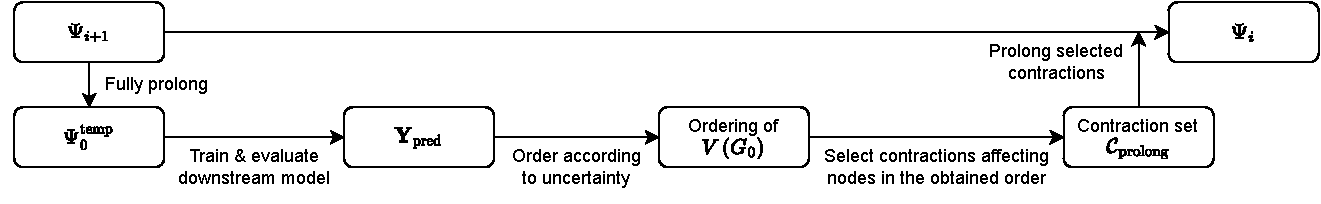
\includegraphics[width=\textwidth]{images/adaptive-prolongation/adaptive-prolongation.pdf}
	\caption{A schematic explanation of the adaptive prolongation algorithm for obtaining the embedding \( \Psi_{i} \) from \( \Psi_{i + 1} \).}
	\label{fig:adaptive-prolongation}
\end{figure}

Let us denote \( \Psi_K, \dots, \Psi_0 \) the resulting embedding sequence. Similarly to standard HARP prolongation, the algorithm starts with the coarsest graph \( G_L \), trains a graph model to compute its embedding \( \Psi_K \) and gradually refines it until reaching the embedding \( \Psi_0 \). These prolongation steps are interlaid with continued training of the graph model, as in standard HARP. A description of a single prolongation step from \( \Psi_{i + 1} \) to \( \Psi_i \) follows, is schematically outlined in Figure~\ref{fig:adaptive-prolongation} and described in detail in Algorithm \ref{alg:adaptive-prolongation}.

% TODO: Add line numbers and link to them from the text
\begin{algorithm*}
  \caption{Adaptive prolongation}
  \label{alg:adaptive-prolongation}
  \begin{algorithmic}
    \Require $ G_0 $ \Comment The original graph
    \Require $ \bm{y}_\mathrm{train} $ \Comment Training labels
    \Require $ n_p $ \Comment The number of nodes to prolong
    \Require $ \Psi_{i + 1} $ \Comment The previous embedding
    \Require $ \mathcal{C}_L^{(i + 1)}, \dots, \mathcal{C}_0^{(i + 1)} $ \Comment A list of all the contractions yet to be reversed
    \Ensure $ \Psi_i $ \Comment The next embedding
    \Ensure $ \mathcal{C}_L^{(i)}, \dots, \mathcal{C}_0^{(i)} $ \Comment Updated contraction list without the prolonged contractions
    \Statex
    \State $ node\_order \gets \Call{get\_node\_order}{G_0, \Psi_{i+1}, \bm{y}_\mathrm{train}, \mathcal{C}_L^{(i + 1)}, \dots, \mathcal{C}_0^{(i + 1)}} $
    \State $ \mathcal{C}_\mathrm{prolong} \gets \Call{select\_contractions}{node\_order, n_p, \mathcal{C}_L^{(i + 1)}, \dots, \mathcal{C}_0^{(i + 1)}} $
    \State $ \Psi_i \gets $ use $ \mathcal{C}_\mathrm{prolong} $ to prolong the embedding $ \Psi_{i + 1} $
    \State $ \mathcal{C}_L^{(i)}, \dots, \mathcal{C}_0^{(i)} \gets $ remove contractions in $ \mathcal{C}_\mathrm{prolong} $ from $ \mathcal{C}_L^{(i + 1)}, \dots, \mathcal{C}_0^{(i + 1)} $
    \Statex
    \Function{get\_node\_order}{$ G_0, \Psi_{i+1}, \bm{y}_\mathrm{train}, \mathcal{C}_L^{(i + 1)}, \dots, \mathcal{C}_0^{(i + 1)} $}
        \State $ \Psi_0^\mathrm{temp} \gets $ use $ \mathcal{C}_L^{(i + 1)}, \dots, \mathcal{C}_0^{(i + 1)} $ to fully prolong the current embedding $ \Psi_{i+1} $ to $ G_0 $
        \State $ model \gets \Call{train\_downstream\_model}{\Psi_0^\mathrm{temp}, \bm{y}_\mathrm{train}} $
        \State $ \mathmat{Y}_\mathrm{pred} \gets \Call{predict}{model, node} $ for each $ node \in V \left( G_0 \right) $
        \State $ entropy\_per\_node \gets H \left( \mathmat{Y}_\mathrm{pred} \right) $
        \State \Return $ V \left( G_0 \right) $, sorted in descending order by $ entropy\_per\_node $
    \EndFunction
    \Statex
    \Function{select\_contractions}{$ ordered\_nodes, n_p, \mathcal{C}_L^{(i + 1)}, \dots, \mathcal{C}_0^{(i + 1)} $}
        \State $ \mathcal{C}_\mathrm{prolong} \gets \left\{ \right\} $
        \For{$ node \in ordered\_nodes $, \textbf{until} $ \left\lvert \mathcal{C}_\mathrm{prolong} \right\rvert = n_p $}
            \State $ contraction \gets \Call{resolve\_contraction}{node, \mathcal{C}_\mathrm{prolong}, \mathcal{C}_L^{(i + 1)}, \dots, \mathcal{C}_0^{(i + 1)}} $
            \State If $ contraction \neq \mathrm{null} $, add $ contraction $ to $ \mathcal{C}_\mathrm{prolong} $
        \EndFor
        \State \Return $ \mathcal{C}_\mathrm{prolong} $
    \EndFunction
    \Statex
    \Function{resolve\_contraction}{$ node, \mathcal{C}_\mathrm{prolong}, \mathcal{C}_L^{(i + 1)}, \dots, \mathcal{C}_0^{(i + 1)} $}
        \State $ contraction \gets \mathrm{null} $
        \For{$ j \in \left\{ 0, \dots, L \right\} $} \Comment I.e. all steps of the original coarsening from finest to coarsest
            \State $ contraction\_candidate \gets $ find in $ \mathcal{C}_j^{(i + 1)} $ a contraction that affects $ node $, if not found, continue with $ j + 1 $
            \If{$ contraction\_candidate \in \mathcal{C}_\mathrm{prolong} $}
                \State \Return $ contraction $
            \EndIf
            \State $ contraction \gets contraction\_candidate $
            \State $ node \gets $ apply $ contraction $ to $ node $, so that in the next loop, a subsequent contraction may be selected
        \EndFor
        \State \Return $ contraction $
    \EndFunction
  \end{algorithmic}
\end{algorithm*}

The procedure keeps track of all the edge contractions that were made in the dataset augmentation part of the algorithm and gradually reverses them. To this end, apart from the embedding \( \Psi_i \), the set of all contractions yet to be reversed as of step \( i \) is kept as \( \mathcal{C}_L^{(i)}, \dots, \mathcal{C}_0^{(i)} \), with the initial values \( \mathcal{C}_j^{(K)} \) corresponding to the underlying coarsening \( \varphi_j \) as defined in Section~\ref{sec:harp}.

In each prolongation step, the embedding \( \Psi_{i + 1} \) is prolonged to \( \Psi_i \) by selecting a set of \( n_p \) contractions \( \mathcal{C}_\mathrm{prolong} \) and undoing them by copying and reusing the embedding of the node resulting from the contraction to both of the contracted nodes. To obtain \( \mathcal{C}_\mathrm{prolong} \), nodes of \( G_0 \) are first ordered in such a way that corresponds to the usefulness of prolonging them. Subsequently, the set \( \mathcal{C}_L^{(i + 1)}, \dots, \mathcal{C}_0^{(i + 1)} \) is ordered to match this node ordering by considering the nodes that the individual contractions affect. \( \mathcal{C}_\mathrm{prolong} \) is then selected by taking the first \( n_p \) contractions. If multiple contractions affecting the same node are available in the sequence \( \mathcal{C}_L^{(i + 1)}, \dots, \mathcal{C}_0^{(i + 1)} \), one is selected from \( \mathcal{C}_j^{(i + 1)} \) corresponding to the coarsest-level coarsening. The sequence \( \mathcal{C}_L^{(i)}, \dots, \mathcal{C}_0^{(i)} \) is produced from \( \mathcal{C}_L^{(i + 1)}, \dots, \mathcal{C}_0^{(i + 1)} \) by removing all of the edges contained in \( \mathcal{C}_\mathrm{prolong} \).

To obtain an ordering of nodes of \( G_0 \) based on the usefulness of their prolongation, the embedding \( \Psi_{i + 1} \) is fully prolonged to a temporary embedding of the full graph, \( \Psi_0^\mathrm{temp} \). The downstream model is then trained using this temporary embedding to obtain \( \mathmat{Y}_\mathrm{pred} \), the predicted posterior distribution of classes for each node in \( G_0 \) (e.g. the output of the softmax layer of an MLP). The entropy of this distribution is measured, representing the amount of uncertainty in the classifier for each given node. The nodes are ordered based on the entropy from highest to lowest. This reflects the principle that it is most useful to prolong those nodes where the downstream classifier is the least certain. For downstream tasks other than node classification, the ordering would need to be defined in a different manner (for example using labels, which are not available for all nodes in our case), however the approach of prolonging the nodes about which the downstream model is the most uncertain can be extended to other tasks.
